\documentclass{standalone}
\usepackage{tikz}
\usetikzlibrary{patterns, positioning}
\usepackage[sfdefault]{ClearSans} %% option 'sfdefault' activates Clear Sans as the default text font
\usepackage[T1]{fontenc}

\begin{document}
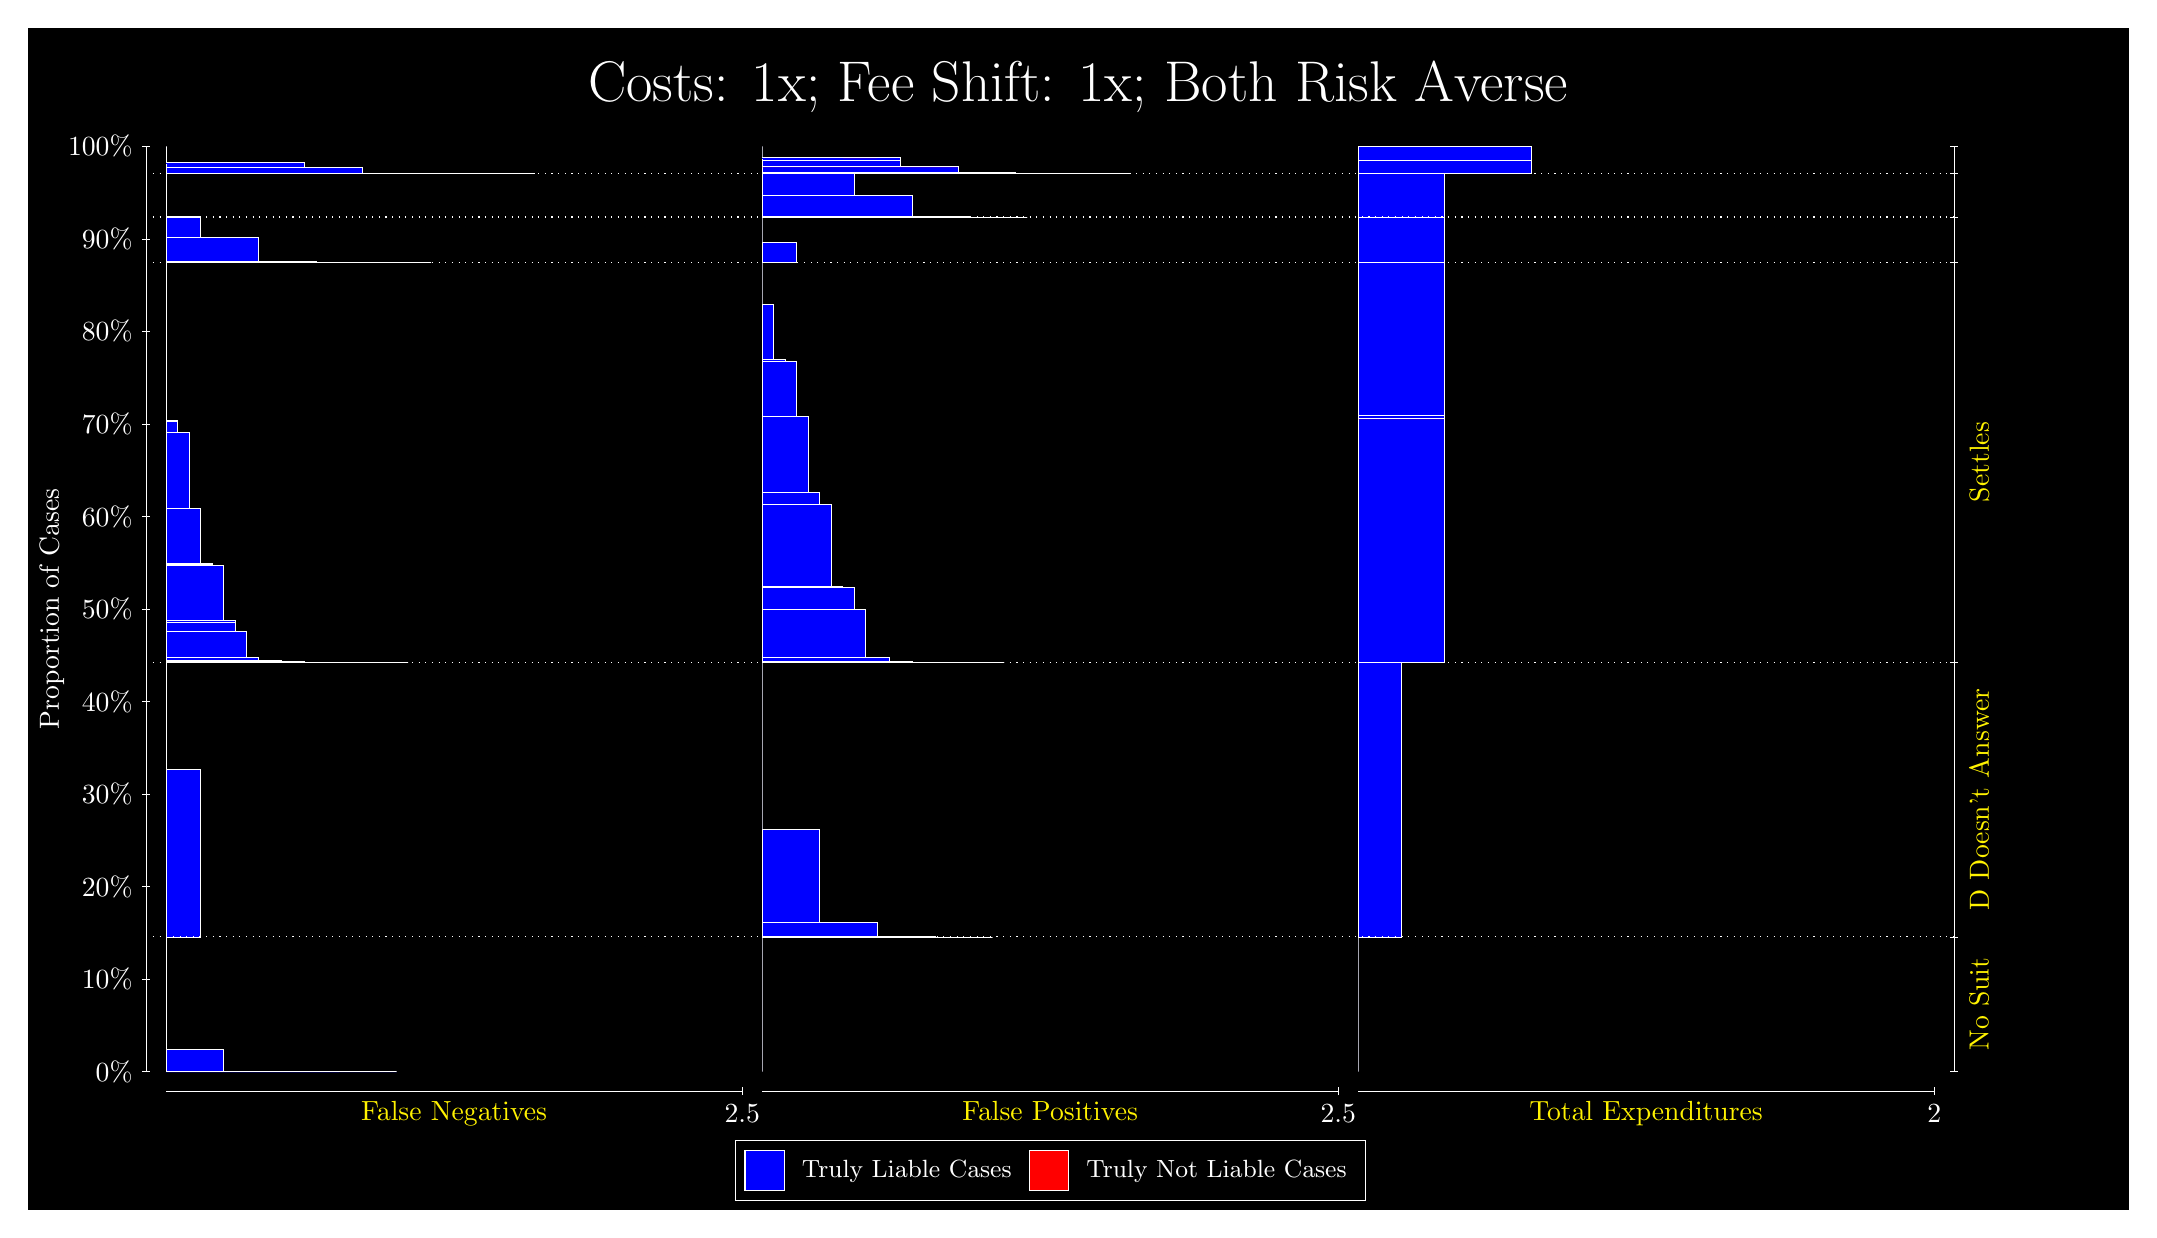
\begin{tikzpicture}
\draw[fill=black] (0,0) rectangle (26.667,15);
\draw[text=white] (0,13.5) rectangle (26.667,15) node[midway] {\huge Costs: 1x; Fee Shift: 1x; Both Risk Averse};
\draw[white, very thin] (1.5,1.75) -- (1.5,13.5);
\node[rotate=90, text=white, anchor=center] at (0.3, 7.625) {Proportion of Cases};
\draw[white, very thin] (1.45,1.75) -- (1.55,1.75);
\node[text=white, anchor=east] at (1.45, 1.75) {0\%};
\draw[white, very thin] (1.45,2.925) -- (1.55,2.925);
\node[text=white, anchor=east] at (1.45, 2.925) {10\%};
\draw[white, very thin] (1.45,4.1) -- (1.55,4.1);
\node[text=white, anchor=east] at (1.45, 4.1) {20\%};
\draw[white, very thin] (1.45,5.275) -- (1.55,5.275);
\node[text=white, anchor=east] at (1.45, 5.275) {30\%};
\draw[white, very thin] (1.45,6.45) -- (1.55,6.45);
\node[text=white, anchor=east] at (1.45, 6.45) {40\%};
\draw[white, very thin] (1.45,7.625) -- (1.55,7.625);
\node[text=white, anchor=east] at (1.45, 7.625) {50\%};
\draw[white, very thin] (1.45,8.8) -- (1.55,8.8);
\node[text=white, anchor=east] at (1.45, 8.8) {60\%};
\draw[white, very thin] (1.45,9.975) -- (1.55,9.975);
\node[text=white, anchor=east] at (1.45, 9.975) {70\%};
\draw[white, very thin] (1.45,11.15) -- (1.55,11.15);
\node[text=white, anchor=east] at (1.45, 11.15) {80\%};
\draw[white, very thin] (1.45,12.325) -- (1.55,12.325);
\node[text=white, anchor=east] at (1.45, 12.325) {90\%};
\draw[white, very thin] (1.45,13.5) -- (1.55,13.5);
\node[text=white, anchor=east] at (1.45, 13.5) {100\%};

\draw[white, very thin] (24.457,1.75) -- (24.457,13.5);
\draw[white, very thin] (24.407,1.75) -- (24.507,1.75);
\node[anchor=west] at (24.407, 1.75) {};
\draw[white, very thin] (24.407,3.4602) -- (24.507,3.4602);
\node[anchor=west] at (24.407, 3.4602) {};
\draw[white, very thin] (24.407,6.9492) -- (24.507,6.9492);
\node[anchor=west] at (24.407, 6.9492) {};
\draw[white, very thin] (24.407,12.03) -- (24.507,12.03);
\node[anchor=west] at (24.407, 12.03) {};
\draw[white, very thin] (24.407,12.603) -- (24.507,12.603);
\node[anchor=west] at (24.407, 12.603) {};
\draw[white, very thin] (24.407,13.159) -- (24.507,13.159);
\node[anchor=west] at (24.407, 13.159) {};
\draw[white, very thin] (24.407,13.5) -- (24.507,13.5);
\node[anchor=west] at (24.407, 13.5) {};

\draw[white, very thin, fill=blue] (1.75,1.75) rectangle (4.6775,1.75);
\draw[white, very thin, fill=blue] (1.75,1.75) rectangle (3.9457,1.75);
\draw[white, very thin, fill=blue] (1.75,1.75) rectangle (3.2138,1.7524);
\draw[white, very thin, fill=blue] (1.75,1.7524) rectangle (2.4819,2.03);
\draw[white, very thin, fill=red] (1.75,2.03) rectangle (1.75,2.03);
\draw[white, very thin, fill=blue] (1.75,2.03) rectangle (1.75,3.4602);
\draw[white, very thin, fill=blue] (1.75,3.4602) rectangle (2.1891,5.5866);
\draw[white, very thin, fill=red] (1.75,5.5866) rectangle (1.75,5.5866);
\draw[white, very thin, fill=blue] (1.75,5.5866) rectangle (1.75,6.9492);
\draw[white, very thin, fill=blue] (1.75,6.9492) rectangle (4.8239,6.9492);
\draw[white, very thin, fill=blue] (1.75,6.9492) rectangle (4.5312,6.9492);
\draw[white, very thin, fill=blue] (1.75,6.9492) rectangle (4.2384,6.9492);
\draw[white, very thin, fill=blue] (1.75,6.9492) rectangle (4.092,6.9492);
\draw[white, very thin, fill=blue] (1.75,6.9492) rectangle (3.9457,6.9492);
\draw[white, very thin, fill=blue] (1.75,6.9492) rectangle (3.7993,6.9492);
\draw[white, very thin, fill=blue] (1.75,6.9492) rectangle (3.6529,6.9492);
\draw[white, very thin, fill=blue] (1.75,6.9492) rectangle (3.5065,6.9571);
\draw[white, very thin, fill=blue] (1.75,6.9571) rectangle (3.3602,6.958);
\draw[white, very thin, fill=blue] (1.75,6.958) rectangle (3.2138,6.9755);
\draw[white, very thin, fill=blue] (1.75,6.9755) rectangle (3.0674,6.9755);
\draw[white, very thin, fill=blue] (1.75,6.9755) rectangle (3.0674,6.9761);
\draw[white, very thin, fill=blue] (1.75,6.9761) rectangle (2.921,7.0065);
\draw[white, very thin, fill=blue] (1.75,7.0065) rectangle (2.7746,7.3439);
\draw[white, very thin, fill=blue] (1.75,7.3439) rectangle (2.6283,7.4522);
\draw[white, very thin, fill=blue] (1.75,7.4522) rectangle (2.6283,7.4784);
\draw[white, very thin, fill=blue] (1.75,7.4784) rectangle (2.4819,8.1821);
\draw[white, very thin, fill=blue] (1.75,8.1821) rectangle (2.3355,8.1962);
\draw[white, very thin, fill=blue] (1.75,8.1962) rectangle (2.3355,8.2076);
\draw[white, very thin, fill=blue] (1.75,8.2076) rectangle (2.1891,8.9024);
\draw[white, very thin, fill=blue] (1.75,8.9024) rectangle (2.0428,9.8697);
\draw[white, very thin, fill=blue] (1.75,9.8697) rectangle (1.8964,10.006);
\draw[white, very thin, fill=blue] (1.75,10.006) rectangle (1.8964,10.027);
\draw[white, very thin, fill=red] (1.75,10.027) rectangle (1.75,10.027);
\draw[white, very thin, fill=blue] (1.75,10.027) rectangle (1.75,12.03);
\draw[white, very thin, fill=blue] (1.75,12.03) rectangle (5.1167,12.03);
\draw[white, very thin, fill=blue] (1.75,12.03) rectangle (4.3848,12.03);
\draw[white, very thin, fill=blue] (1.75,12.03) rectangle (3.6529,12.037);
\draw[white, very thin, fill=blue] (1.75,12.037) rectangle (2.921,12.345);
\draw[white, very thin, fill=blue] (1.75,12.345) rectangle (2.1891,12.603);
\draw[white, very thin, fill=red] (1.75,12.603) rectangle (1.75,12.603);
\draw[white, very thin, fill=blue] (1.75,12.603) rectangle (2.1891,12.606);
\draw[white, very thin, fill=red] (1.75,12.606) rectangle (1.75,12.606);
\draw[white, very thin, fill=blue] (1.75,12.606) rectangle (1.75,13.159);
\draw[white, very thin, fill=blue] (1.75,13.159) rectangle (6.4341,13.159);
\draw[white, very thin, fill=blue] (1.75,13.159) rectangle (5.7022,13.159);
\draw[white, very thin, fill=blue] (1.75,13.159) rectangle (4.9703,13.164);
\draw[white, very thin, fill=blue] (1.75,13.164) rectangle (4.2384,13.234);
\draw[white, very thin, fill=blue] (1.75,13.234) rectangle (3.9457,13.234);
\draw[white, very thin, fill=blue] (1.75,13.234) rectangle (3.5065,13.293);
\draw[white, very thin, fill=blue] (1.75,13.293) rectangle (3.2138,13.293);
\draw[white, very thin, fill=blue] (1.75,13.293) rectangle (2.7746,13.294);
\draw[white, very thin, fill=blue] (1.75,13.294) rectangle (2.4819,13.302);
\draw[white, very thin, fill=blue] (1.75,13.302) rectangle (2.0428,13.302);
\draw[white, very thin, fill=red] (1.75,13.302) rectangle (1.75,13.302);
\draw[white, very thin, fill=blue] (1.75,13.302) rectangle (1.75,13.5);
\draw[white, very thin, fill=red] (9.3189,1.75) rectangle (9.3189,1.75);
\draw[white, very thin, fill=blue] (9.3189,1.75) rectangle (9.3189,3.4602);
\draw[white, very thin, fill=red] (9.3189,3.4602) rectangle (12.246,3.4602);
\draw[white, very thin, fill=blue] (9.3189,3.4602) rectangle (12.246,3.4602);
\draw[white, very thin, fill=blue] (9.3189,3.4602) rectangle (11.515,3.4615);
\draw[white, very thin, fill=blue] (9.3189,3.4615) rectangle (10.783,3.6492);
\draw[white, very thin, fill=blue] (9.3189,3.6492) rectangle (10.051,4.8227);
\draw[white, very thin, fill=blue] (9.3189,4.8227) rectangle (9.3189,6.9492);
\draw[white, very thin, fill=red] (9.3189,6.9492) rectangle (12.393,6.9492);
\draw[white, very thin, fill=blue] (9.3189,6.9492) rectangle (12.393,6.9492);
\draw[white, very thin, fill=red] (9.3189,6.9492) rectangle (11.807,6.9492);
\draw[white, very thin, fill=blue] (9.3189,6.9492) rectangle (11.807,6.9492);
\draw[white, very thin, fill=blue] (9.3189,6.9492) rectangle (11.661,6.9492);
\draw[white, very thin, fill=red] (9.3189,6.9492) rectangle (11.515,6.9492);
\draw[white, very thin, fill=blue] (9.3189,6.9492) rectangle (11.515,6.9492);
\draw[white, very thin, fill=red] (9.3189,6.9492) rectangle (11.222,6.9492);
\draw[white, very thin, fill=blue] (9.3189,6.9492) rectangle (11.222,6.9588);
\draw[white, very thin, fill=blue] (9.3189,6.9588) rectangle (11.075,6.9588);
\draw[white, very thin, fill=red] (9.3189,6.9588) rectangle (10.929,6.9588);
\draw[white, very thin, fill=blue] (9.3189,6.9588) rectangle (10.929,7.0075);
\draw[white, very thin, fill=blue] (9.3189,7.0075) rectangle (10.783,7.009);
\draw[white, very thin, fill=red] (9.3189,7.009) rectangle (10.636,7.009);
\draw[white, very thin, fill=blue] (9.3189,7.009) rectangle (10.636,7.6233);
\draw[white, very thin, fill=blue] (9.3189,7.6233) rectangle (10.49,7.8989);
\draw[white, very thin, fill=red] (9.3189,7.8989) rectangle (10.344,7.8989);
\draw[white, very thin, fill=blue] (9.3189,7.8989) rectangle (10.344,7.9138);
\draw[white, very thin, fill=blue] (9.3189,7.9138) rectangle (10.197,8.9522);
\draw[white, very thin, fill=red] (9.3189,8.9522) rectangle (10.051,8.9522);
\draw[white, very thin, fill=blue] (9.3189,8.9522) rectangle (10.051,9.1092);
\draw[white, very thin, fill=blue] (9.3189,9.1092) rectangle (9.9044,10.076);
\draw[white, very thin, fill=blue] (9.3189,10.076) rectangle (9.758,10.771);
\draw[white, very thin, fill=blue] (9.3189,10.771) rectangle (9.6116,10.797);
\draw[white, very thin, fill=blue] (9.3189,10.797) rectangle (9.4652,11.5);
\draw[white, very thin, fill=blue] (9.3189,11.5) rectangle (9.3189,12.03);
\draw[white, very thin, fill=red] (9.3189,12.03) rectangle (9.758,12.03);
\draw[white, very thin, fill=blue] (9.3189,12.03) rectangle (9.758,12.287);
\draw[white, very thin, fill=blue] (9.3189,12.287) rectangle (9.3189,12.603);
\draw[white, very thin, fill=red] (9.3189,12.603) rectangle (12.686,12.603);
\draw[white, very thin, fill=blue] (9.3189,12.603) rectangle (12.686,12.603);
\draw[white, very thin, fill=blue] (9.3189,12.603) rectangle (11.954,12.606);
\draw[white, very thin, fill=blue] (9.3189,12.606) rectangle (11.222,12.884);
\draw[white, very thin, fill=blue] (9.3189,12.884) rectangle (10.49,13.156);
\draw[white, very thin, fill=blue] (9.3189,13.156) rectangle (9.758,13.159);
\draw[white, very thin, fill=red] (9.3189,13.159) rectangle (14.003,13.159);
\draw[white, very thin, fill=blue] (9.3189,13.159) rectangle (14.003,13.159);
\draw[white, very thin, fill=red] (9.3189,13.159) rectangle (13.271,13.159);
\draw[white, very thin, fill=blue] (9.3189,13.159) rectangle (13.271,13.159);
\draw[white, very thin, fill=red] (9.3189,13.159) rectangle (12.539,13.159);
\draw[white, very thin, fill=blue] (9.3189,13.159) rectangle (12.539,13.166);
\draw[white, very thin, fill=blue] (9.3189,13.166) rectangle (11.807,13.243);
\draw[white, very thin, fill=red] (9.3189,13.243) rectangle (11.807,13.243);
\draw[white, very thin, fill=blue] (9.3189,13.243) rectangle (11.807,13.244);
\draw[white, very thin, fill=blue] (9.3189,13.244) rectangle (11.075,13.322);
\draw[white, very thin, fill=blue] (9.3189,13.322) rectangle (11.075,13.357);
\draw[white, very thin, fill=red] (9.3189,13.357) rectangle (10.783,13.357);
\draw[white, very thin, fill=blue] (9.3189,13.357) rectangle (10.783,13.357);
\draw[white, very thin, fill=blue] (9.3189,13.357) rectangle (10.344,13.358);
\draw[white, very thin, fill=blue] (9.3189,13.358) rectangle (10.344,13.365);
\draw[white, very thin, fill=red] (9.3189,13.365) rectangle (10.051,13.365);
\draw[white, very thin, fill=blue] (9.3189,13.365) rectangle (10.051,13.366);
\draw[white, very thin, fill=blue] (9.3189,13.366) rectangle (9.6116,13.366);
\draw[white, very thin, fill=blue] (9.3189,13.366) rectangle (9.6116,13.366);
\draw[white, very thin, fill=red] (9.3189,13.366) rectangle (9.3189,13.366);
\draw[white, very thin, fill=blue] (9.3189,13.366) rectangle (9.3189,13.5);
\draw[white, very thin, fill=red] (16.888,1.75) rectangle (16.888,1.75);
\draw[white, very thin, fill=blue] (16.888,1.75) rectangle (16.888,3.4602);
\draw[white, very thin, fill=red] (16.888,3.4602) rectangle (17.437,3.4602);
\draw[white, very thin, fill=blue] (16.888,3.4602) rectangle (17.437,6.9492);
\draw[white, very thin, fill=red] (16.888,6.9492) rectangle (17.986,6.9492);
\draw[white, very thin, fill=blue] (16.888,6.9492) rectangle (17.986,10.042);
\draw[white, very thin, fill=red] (16.888,10.042) rectangle (17.986,10.042);
\draw[white, very thin, fill=blue] (16.888,10.042) rectangle (17.986,10.09);
\draw[white, very thin, fill=red] (16.888,10.09) rectangle (17.986,10.09);
\draw[white, very thin, fill=blue] (16.888,10.09) rectangle (17.986,12.03);
\draw[white, very thin, fill=red] (16.888,12.03) rectangle (17.986,12.03);
\draw[white, very thin, fill=blue] (16.888,12.03) rectangle (17.986,12.603);
\draw[white, very thin, fill=red] (16.888,12.603) rectangle (17.986,12.603);
\draw[white, very thin, fill=blue] (16.888,12.603) rectangle (17.986,13.159);
\draw[white, very thin, fill=red] (16.888,13.159) rectangle (19.083,13.159);
\draw[white, very thin, fill=blue] (16.888,13.159) rectangle (19.083,13.322);
\draw[white, very thin, fill=red] (16.888,13.322) rectangle (19.083,13.322);
\draw[white, very thin, fill=blue] (16.888,13.322) rectangle (19.083,13.5);
\draw[white, dotted] (1.5,3.4602) -- (24.457,3.4602);
\draw[white, dotted] (1.5,6.9492) -- (24.457,6.9492);
\draw[white, dotted] (1.5,12.03) -- (24.457,12.03);
\draw[white, dotted] (1.5,12.603) -- (24.457,12.603);
\draw[white, dotted] (1.5,13.159) -- (24.457,13.159);
\draw[white, very thin] (1.75,1.5) -- (9.0689,1.5);
\node[text=yellow, anchor=north] at (5.4094, 1.5) {False Negatives};
\draw[white, very thin] (9.0689,1.45) -- (9.0689,1.55);
\node[text=white, anchor=north] at (9.0689, 1.45) {2.5};

\draw[white, very thin] (9.3189,1.5) -- (16.638,1.5);
\node[text=yellow, anchor=north] at (12.978, 1.5) {False Positives};
\draw[white, very thin] (16.638,1.45) -- (16.638,1.55);
\node[text=white, anchor=north] at (16.638, 1.45) {2.5};

\draw[white, very thin] (16.888,1.5) -- (24.207,1.5);
\node[text=yellow, anchor=north] at (20.547, 1.5) {Total Expenditures};
\draw[white, very thin] (24.207,1.45) -- (24.207,1.55);
\node[text=white, anchor=north] at (24.207, 1.45) {2};

\node[text=yellow, centered, rotate=90] at (24.777, 2.6051) {No Suit};
\node[text=yellow, centered, rotate=90] at (24.777, 5.2047) {D Doesn't Answer};
\node[text=yellow, centered, rotate=90] at (24.777, 9.4894) {Settles};




\draw (12.978300999999998,1.5) node[draw=none] (baseCoordinate) {};
\begin{scope}[align=center]
        \matrix[scale=0.5, draw=white, below=0.5cm of baseCoordinate, nodes={draw}, column sep=0.1cm]{
            \node[rectangle, draw, minimum width=0.5cm, minimum height=0.5cm, fill=blue] {}; &
            \node[draw=none, font=\small, text=white] (B) {Truly Liable Cases}; &
            \node[rectangle, draw, minimum width=0.5cm, minimum height=0.5cm, fill=red] {}; &
            \node[draw=none, font=\small, text=white] (B) {Truly Not Liable Cases}; \\
            };
\end{scope}

\end{tikzpicture}
\end{document}